\documentclass{article}
\usepackage{geometry}
\usepackage{graphicx}
\usepackage{hyperref}
\usepackage{listings}
\usepackage{color}
\usepackage{amsmath}
\usepackage{titlesec}
\usepackage{titling}
\usepackage{dirtree}

\definecolor{lightgray}{rgb}{.9,.9,.9}
\definecolor{darkgray}{rgb}{.4,.4,.4}
\definecolor{purple}{rgb}{0.65, 0.12, 0.82}
\lstdefinelanguage{JavaScript}{
  keywords={break, case, catch, continue, debugger, default, delete, do, else, false, finally, for, function, if, in, instanceof, new, null, return, switch, this, throw, true, try, typeof, var, void, while, with},
  morecomment=[l]{//},
  morecomment=[s]{/*}{*/},
  morestring=[b]',
  morestring=[b]",
  ndkeywords={class, export, boolean, throw, implements, import, this},
  keywordstyle=\color{blue}\bfseries,
  ndkeywordstyle=\color{darkgray}\bfseries,
  identifierstyle=\color{black},
  commentstyle=\color{purple}\ttfamily,
  stringstyle=\color{red}\ttfamily,
  sensitive=true
}

\lstset{
   language=JavaScript,
   backgroundcolor=\color{lightgray},
   extendedchars=true,
   basicstyle=\footnotesize\ttfamily,
   showstringspaces=false,
   showspaces=false,
   numbers=left,
   numberstyle=\footnotesize,
   numbersep=9pt,
   tabsize=2,
   breaklines=true,
   showtabs=false,
   captionpos=b
}


\title{\textbf{{\Huge GameMon Documentation}}}
\author{{\Large Josephine Chen, Eric Forsell, Kevin Jang, Andy Walz}}
\date{February 2, 2017}

\begin{document}
\begin{titlepage}
\setlength{\parindent}{0pt}
\setlength{\parskip}{0pt}
\vspace*{\stretch{1}}
\rule{\linewidth}{1pt}
\begin{center}
\Huge GameMon Documentation \\[14pt]
\end{center}
\rule{\linewidth}{2pt}
\begin{center}
\Large Josephine Chen, \\Eric Forsell, \\Kevin Jang, \\Andy Walz \\
\end{center}
\vspace*{\stretch{2}}
Hack Reactor HRR21 Towering-Cranes
\end{titlepage}

\tableofcontents
\newpage

\section{Introduction}
Welcome to GameMon! We hope this documentation helps you navigate around the project quickly and efficiently. GameMon is an app for tracking what video games you have in your collection. Users signup and build out a collection based on the thousands of games available in the GiantBomb API.
\section{File Structure}
\dirtree{%
  .1 towering-cranes.
  .2 client.
  .3 assets.
  .4 andy.jpg.
  .4 eric.jpg.
  .4 favicon.ico.
  .4 gamemon-collection.png.
  .4 gamemon-details.png.
  .4 gamemon-search.png.
  .4 josephine.jpg.
  .4 kevin.jpg.
  .4 Octocat.png.
  .3 home.
  .4 home.html.
  .3 main.
  .4 gameCollection.js.
  .4 main.html.
  .4 search.js.
  .4 selectedGame.js.
  .3 styles.
  .4 styles.css.
  .3 users.
  .4 lock.js.
  .4 signin.html.
  .4 signup.html.
  .3 app.js.
  .3 index.html.
  .2 documentation.
  .3 documentation.pdf.
  .3 documentation.tex.
  .3 documentation.toc.
  .2 node\_modules.
  .2 server.
  .3 config.
  .4 keys.js.
  .3 database.
  .4 databaseHelpers.js.
  .4 db.js.
  .3 giantBomb.
  .4 giantBombHelpers.js.
  .3 server.js.
  .2 .gitignore.
  .2 \_.editorconfig.
  .2 \_.gitattributes.
  .2 \_.gitignore.
  .2 \_.jshintrc.
  .2 \_.travis.yml.
  .2 \_CONTRIBUTING.md.
  .2 \_PRESS-RELEASE.md.
  .2 \_STYLE-GUIDE.md.
  .2 package.json.
  .2 README.md.
}
\section{Database Schema}
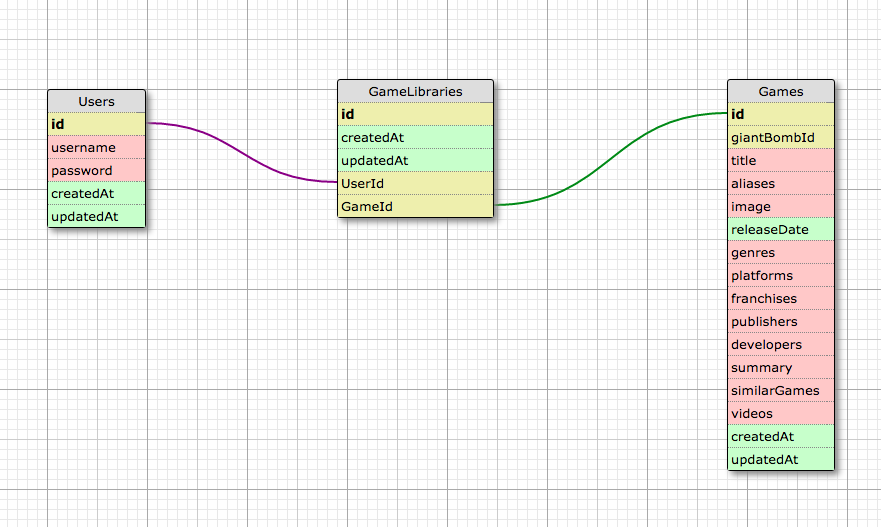
\includegraphics[scale=.5]{Schemav4}

\section{Server-Side}
Server-side files hold the routes and the helper functions needed for the routing.
\subsection{Routes}
\textbf{Database Routes}
\begin{itemize}
  \item '/users'
  \begin{itemize}
    \item POST - receives a username and password from the client and adds each to the database for a specific user
  \end{itemize}
  \item '/games'
  \begin{itemize}
    \item POST - receives a user and a game from the client and adds the game to that user's collection in the database
    \item DELETE - receives a game title and a user from the request body and removes the game from the user’s collection
    \item GET - receives a username from the client as a parameter in the url and sends all of that user’s games back to the client
  \end{itemize}
\end{itemize}
\textbf{Giant Bomb API Routes}
\begin{itemize}
  \item '/games/search/keyword/:keyword'
  \begin{itemize}
    \item GET - receives a keyword from the client as a parameter and returns up to 10 games that match the keyword
  \end{itemize}
  \item '/games/search/id/:id'
  \begin{itemize}
    \item GET - receives a game id from the client as a parameter and returns up to 10 games that match the id
  \end{itemize}
\end{itemize}

\subsection{Database Helper Functions}
\begin{itemize}
  \item createUser - receives a user object from the server and either finds a user with that existing name or creates a new user
  \item addGameToCollection - receives a username and a game object and adds the game to the specified user’s collection.
  \item getGamesFromCollection - receives a username from the server and finds/returns all of that user’s games.
  \item removeGameFromCollection - receives a username and a game from the server and deletes that game from the specified user’s collection
\end{itemize}

\subsection{Giant Bomb API Helper Functions}
Note: ES6 syntax used here in the request calls
\begin{itemize}
  \item searchForGames - receives a search term and uses express’s request module to send that request to the Giant Bomb api.
  \begin{itemize}
    \item \sloppy Example: To search for all Pokemon games our url in the options object would be the following:
   `http://www.giantbomb.com/api/search/?api\_key=\${YOUR-API-KEY}\&format=json\&query="\${pokemon}"\&resources=game`
 \end{itemize}
  \item getGameById - receives an id from and uses that id to get the game with the corresponding id form Giant Bomb.
  \begin{itemize}
    \item \sloppy Example: To search for metroid prime and list its genres and name based on id do the following:
   `http://www.giantbomb.com/api/game/3030-4725/?api\_key=\${YOUR-API-KEY}\&format=json\&field\_list=genres,name`
 \end{itemize}
\end{itemize}

\section{Client-Side}
Front-end uses AngularJS with Materialize/Angular-materialize. Materialize/Angular-materialize can be substituted with Bootstrap or any other front-end framework. Angular-materialize is a set of AngularJS directives to use features in Materialize that requires jQuery. It is NOT the same as Angular Material.
\\
\textbf{Resources:}
\begin{itemize}
  \item \href {https://docs.angularjs.org/api}{AngularJS}
  \item \href {https://krescruz.github.io/angular-materialize/}{Angular-materialize}
  \item \href {https://getmdl.io/started/}{Material Icons}
  \item \href {http://materializecss.com/}{Materialize CSS}
\end{itemize}
\subsection{Files}
The roles of the different files are as follows:
\begin{itemize}
  \item /client/styles/styles.css
  \begin{itemize}
    \item Custom stylesheet for overrides and other styles not included in Materialize
  \end{itemize}
  \item /client/assets
  \begin{itemize}
    \item Images and other files to be used across client pages
  \end{itemize}
  \item /client/index.html
  \begin{itemize}
    \item Loads JS libraries
    \item Sets up header, navigation, and footer
  \end{itemize}
  \item /client/app.js
  \begin{itemize}
    \item Handles client side routing to load templates in /client/main or /client/home
  \end{itemize}
  \item /client/home/home.html
  \begin{itemize}
    \item Template for product landing page
    \item Default page if root directory is loaded or if an invalid url is provided
  \end{itemize}
  \item /client/main/main.html
  \begin{itemize}
    \item Uses ternary operator on gameCollection to see if search sidebar should be displayed. If it should be displayed, the column width is set to 8, if not, it is set to 11.
    \item Uses custom filter in gameCollection.js to allow filtering by title, franchise, platform, and genre
    \item Allows collection view to change between list and grid and sort by title or release date
    \item Holds modal markup that appears when a game is clicked on
  \end{itemize}
  \item /client/main/modal.js
  \begin{itemize}
    \item Controller to load data into the scope for modal information
    \begin{itemize}
      \item similar games
    \end{itemize}
  \end{itemize}
  \item /client/main/gameCollection.js
  \begin{itemize}
    \item Holds a factory that allows
    \begin{itemize}
      \item getUserCollection that loads a game collection for the signed-in user
      \item addGameToCollection adds a selected game to the current users collection
      \item removeGameFromCollection removes the selected game from the current users collection
    \end{itemize}
    \item Holds a custom filter that takes in setFilter(filterOpt) as an input where filterOpt is an array
    \begin{itemize}
      \item custom filter checks for a match in the respective locations of all the objects and returns all matches
      \item first element of filterOpt is the search term to find
      \item second element is what type of filter term it is: text, platform, or genre
      \item returns all objects that will be displayed after filtering
      \item items holds all possible objects
    \end{itemize}
  \end{itemize}
  \item /client/main/search.js
  \begin{itemize}
    \item Holds a factory that allows
    \begin{itemize}
      \item searchByTerm
      \item searchById
    \end{itemize}
  \end{itemize}
\end{itemize}
\subsection{User Authentication}
We implemented a client-side authentication using Auth0. The toggle.js files holds the logic for the authentication. First, we instantiate a module gameMon.toggle. We include the dependency 'auth0' in order to use the Angular wrapper for Auth0. We pass the domain and client id in as an argument to authProvider.
\begin{lstlisting}
authProvider.init({
  domain: <our domain key>,
  clientID: <our client ID>
  });
\end{lstlisting}
After this we create a controller, ‘LoginController’, which runs when a user clicks signup and when a user logs out.  The important takeaway from this controller is its use of local storage.  When the user logs in, their profile information and Auth0 access token is added to the browser’s local storage.  We set and remove the profile and token by calling ‘localStorage.setItem’ and ‘localStorage.removeItem’. We are able to keep the user logged in or logged out by looking for a profile on their local browser and toggling the signup/sign out buttons accordingly with ng-if.

\section{Deployment}
Towering-Cranes used \href{http://www.digitalocean.com/}{DigitalOcean} for deployment. The droplet uses a MEAN base image (0.5.0) running on Ubuntu 16.04 with MySQL and several other technologies.

\textbf{It is best to have ONE team member work on deployment. This removes the need for multiple SSH keys and rule out issues with individual development environments.}
\textbf{Steps to get it running (this will help ensure there are no issues):}
\begin{enumerate}
  \item Create Droplet with 1-Click App: MEAN 0.5.0 on 16.04
  \begin{itemize}
    \item Smallest droplet size is fine
    \item Datacenter is whatever you want -- closest to your users is best
    \item \textbf{Add SSH keys here and now!} Adding them later is a headache
  \end{itemize}
  \item After the droplet is created, UPDATE your droplet
  \begin{enumerate}
    \item Log in using root user: \textbf{ssh://root@YOUR\_DROPLET\_IP}
    \begin{itemize}
      \item If you set up ssh keys correctly, the server shouldn't ask for your root password
      \item If you run into problems, use the droplet console via DigitalOcean's dashboard to log in as root and troubleshoot. On the console page, there is also a link to reset root password if necessary
    \end{itemize}
    \item Run the apt-get commands to update
    \begin{enumerate}
      \item \textbf{sudo apt-get upgrade}
      \item \textbf{sudo apt-get update}
    \end{enumerate}
  \end{enumerate}
  \item Add swapfile (\href{https://www.digitalocean.com/community/tutorials/how-to-add-swap-on-ubuntu-14-04}{reference})
  \begin{enumerate}
    \item This is \textbf{necessary} because MySQL needs more RAM than the server has been allocated. Npm install might also fail if the swapfile isn't created
    \item Referencing the link above, run the following commands
    \begin{enumerate}
      \item \textbf{sudo fallocate -l 4G /swapfile}
      \item \textbf{sudo chmod 600 /swapfile}
      \item \textbf{sudo mkswap /swapfile}
      \item \textbf{sudo swapon /swapfile}
      \item \textbf{sudo nano /etc/fstab}
      \item \textbf{sudo sysctl vm.swappiness=10} (persists until system reboot)
      \item \textbf{sudo sysctl vm.vfs\_cache\_pressure=50} (persists until system reboot)
    \end{enumerate}
  \end{enumerate}
  \item Install MySQL (\href{https://www.digitalocean.com/community/tutorials/how-to-install-mysql-on-ubuntu-16-04}{reference})
  \begin{enumerate}
    \item Run the following commands referencing the above link as necessary
    \begin{enumerate}
      \item \textbf{sudo apt-get install mysql-server} This will prompt you to create a root password. Write it down!
      \item \textbf{sudo mysql\_secure\_installation}
    \end{enumerate}
    \item MySQL should be up and running
    \item Log into the MySQL CLI
    \begin{enumerate}
      \item \textbf{mysql -u root -p} (enter password at prompt)
    \end{enumerate}
    \item Create a database named gamemon
    \begin{enumerate}
      \item \textbf{CREATE DATABASE gamemon}
    \end{enumerate}
  \end{enumerate}
  \item Get a Giant Bomb API key (write this down)
  \begin{itemize}
    \item \href{http://www.giantbomb.com/api/}{Giant Bomb API}
  \end{itemize}
  \item Clone repo (with work tree and git tracking separation) (\href{https://www.digitalocean.com/community/tutorials/how-to-set-up-automatic-deployment-with-git-with-a-vps}{reference})
  \begin{enumerate}
    \item Navigate to a directory you want to store both the repo and a separate git folder (towering-cranes used root/)
    \item Install PM2 for running the web app server in the background
    \begin{enumerate}
      \item \textbf{npm install -g pm2}
      \item Create a config file for PM2 with env variables
      \begin{enumerate}
        \item \textbf{touch gamemon.config.js}
        \item \textbf{nano gamemon.config.js}
        \item Copy and paste this replacing the db password and Giant Bomb API key:
        \begin{lstlisting}
        module.exports = {
          /**
           * Application configuration section
           * http://pm2.keymetrics.io/docs/usage/application-declaration/
           */
          apps : [
            {
              name      : "server",
              script    : "node towering-cranes/server/server.js",
              env: {
                PORT: 80,
                DB_PASSWORD: password_here******,
                GIANTBOMB_API_KEY: api_key_here******
              }
            }
          ]
        \end{lstlisting}
        \item Save file
      \end{enumerate}
    \end{enumerate}
    \item Clone the web app repo
    \begin{enumerate}
      \item \textbf{git clone REPO\_LINK\_HERE}
      \item cd into the repo folder
      \item \textbf{npm install}
      \item Run the server by cd to where gamemon.config.js is (probably up one directory)
      \item \textbf{pm2 start gamemon.config.js}
    \end{enumerate}
    \item Create bare git
    \begin{enumerate}
      \item \textbf{cd ..}
      \item \textbf{mkdir SOME\_NAME\_HERE.git}
      \item \textbf{cd SOME\_NAME\_HERE.git}
      \item \textbf{git init --bare}
      \item \textbf{cd hooks}
      \item \textbf{nano post-receive}
      \item Add the following lines to the post-receive file (press Ctrl+X to quit and save)
      \begin{enumerate}
        \item \#!/bin/sh
        \item git --work-tree=PATH\_TO\_REPO\_DIRECTORY --git-dir=PATH\_TO\_BARE\_GIT checkout -f
        \item pm2 stop server
        \item sudo fuser -k 80/tcp
        \item pm2 restart server
      \end{enumerate}
      \item chmod +x post-receive
    \end{enumerate}
    \item Set up local workspace (best for only one team member to do this)
    \begin{enumerate}
      \item cd to your local clone of the repo on the server
      \item Add a remote
      \begin{itemize}
        \item \textbf{git remote add live ssh://root@your\_droplet\_ip/path\_to\_bare\_git}
        \item When deploying, \textbf{git push live master} should push all the recent changes and restart the PM2 server instance
      \end{itemize}
    \end{enumerate}
    \item Sometimes the post-receive hook doesn't instantiate the env vars. A workaround when parts aren't working, e.g. search bar, is to ssh into the droplet and run these commands
    \begin{enumerate}
      \item \textbf{ sudo fuser -k 80/tcp}
      \item \textbf{pm2 restart server}
    \end{enumerate}
  \end{enumerate}
\end{enumerate}

  % \item Set environmental variables
  % \begin{enumerate}
  %   \item cd to /etc/
  %   \item Modify environment file
  %   \begin{enumerate}
  %     \item \textbf{nano environment}
  %   \end{enumerate}
  %   \item Add to environment file
  %   \begin{enumerate}
  %     \item PORT=80
  %     \item DB\_PASSWORD=password\_here
  %     \item GIANTBOMB\_API\_KEY=key\_here
  %   \end{enumerate}
  % \end{enumerate}
  % \end{enumerate}
% \end{enumerate}
% \end{flushleft}
% Occasionally, deploying will cause some features to break unexpectedly. We didn’t figure out why this is but it can be solved by sshing into the server and running:
% \begin{enumerate}
%   \item \textbf{sudo fuser -k 80/tcp (to kill the current server running on port 80)}
%   \item \textbf{pm2 server restart}
% \end{enumerate}

\section{Documentation}
If you haven't noticed already, this document is written using \LaTeX, a typesetting system that is great for technical documents.
  \textbf{Steps to start using \LaTeX:}
  \begin{enumerate}
    \item Download one of the TeX distributions
    \begin{itemize}
      \item For Mac users, go to \href {http://www.tug.org/mactex/}{MacTeX}.
      \item For Windows users, check out \href{https://miktex.org/}{MikTeX} or \href{https://www.tug.org/texlive/}{TeXLive}.
      \item For Linux users, go to \href{https://www.tug.org/texlive/}{TeXLive}
    \end{itemize}
    \item Download a viewer with inverse search
    \begin{itemize}
      \item For Mac users, download \href {http://skim-app.sourceforge.net/}{Skim PDF Viewer}.
      \item For Windows users, download \href {https://www.sumatrapdfreader.org/free-pdf-reader.html}{Sumatra PDF}.
    \end{itemize}
    \item Install one of the LaTeX packages in Sublime (LaTeXTools or LaTeXing)
    \item Build your .tex document and start using \LaTeX!
  \end{enumerate}

% \section{Extra - Delete Later}
% \begin{lstlisting}
% function fibMemoization(n, memo) {
%   memo = memo || {};
%   if (memo[n]) {
%     return memo[n];
%   } else if (n <= 1) {
%     return 1;
%   } else {
%     return memo[n] = fibMemoization(n - 1, memo)+fibMemoization(n - 2, memo);
%   }
% }
% \end{lstlisting}
\end{document}